% Лабораторная работа №1. Анализ молекулярной мишени BCR::ABL1 (WT и T315I)
% Компиляция: pdflatex report.tex  (дважды, из папки report)
\documentclass[12pt,a4paper]{article}

\usepackage[T2A]{fontenc}
\usepackage[utf8]{inputenc}
\usepackage[russian]{babel}
\usepackage[left=2.5cm,right=1.5cm,top=2cm,bottom=2cm]{geometry}
\usepackage{booktabs}
\usepackage{longtable}
\usepackage{array}
\usepackage{tabularx}
\usepackage{graphicx}
\usepackage{seqsplit}
\usepackage{enumitem}
\usepackage{amsmath}
\usepackage{float}
\usepackage{caption}
\usepackage[hidelinks]{hyperref}
\usepackage[expansion=false]{microtype}

\captionsetup{font=small,labelfont=bf}
\setlength{\parindent}{1.25em}
\setlength{\emergencystretch}{3em}
\renewcommand{\arraystretch}{1.2}

\newcolumntype{L}[1]{>{\raggedright\arraybackslash}p{#1}}
\newcommand{\smi}[1]{{\ttfamily\scriptsize\seqsplit{#1}}}
\newcommand{\code}[1]{{\ttfamily #1}}

\title{\textbf{Лабораторная работа №1}\\[4pt]
Анализ молекулярной мишени и доступных данных\\[4pt]
\large Объект исследования: BCR::ABL1 тирозинкиназа --- WT и T315I}
\author{Шпока Владислав, Пясецкий Кирилл\\4 курс, 3 группа}
\date{25 сентября 2026 г.}

\begin{document}
\maketitle

\section*{Цель работы}
Собрать и структурировать основные биологические, структурные и химические данные
по BCR::ABL1, сравнить нативную форму киназного домена (далее WT) и вариант с мутацией
T315I, а также сформировать машиночитаемый набор данных, который будет использоваться
в следующих лабораторных работах.

\section*{Использованные ресурсы}
\begin{center}
\begin{tabular}{L{5cm}L{9.5cm}}
\toprule
\textbf{Ресурс} & \textbf{Адрес} \\
\midrule
UniProt & \url{https://www.uniprot.org/uniprotkb/P00519} \\
RCSB Protein Data Bank & \url{https://www.rcsb.org/} \\
AlphaFold DB & \url{https://alphafold.ebi.ac.uk/entry/P00519} \\
ChEMBL & \url{https://www.ebi.ac.uk/chembl/} \\
BindingDB & \url{https://www.bindingdb.org/} \\
PubChem & \url{https://pubchem.ncbi.nlm.nih.gov/} \\
\bottomrule
\end{tabular}
\end{center}

\bigskip
Все числовые данные в отчёте получены из перечисленных баз; для каждого значения
указан источник (идентификатор записи ChEMBL/PDB/PubChem и первичная публикация).
Выборки из ChEMBL и RCSB выполнялись программно через их публичные REST/GraphQL API;
скрипты приведены в приложении~\ref{app:scripts} и приложены к отчёту в папке
\code{scripts/}. Дата обращения ко всем базам --- 25.09.2026.

\section{Идентификация мишени в UniProt}

В UniProt по запросу \emph{ABL1 human} выбрана рецензируемая (reviewed, Swiss-Prot)
запись \code{ABL1\_HUMAN}, accession \code{P00519}.

\begin{center}
\begin{tabular}{L{4.2cm}L{10.3cm}}
\toprule
\textbf{Параметр} & \textbf{Результат} \\
\midrule
Protein name & Tyrosine-protein kinase ABL1 (EC 2.7.10.2); синонимы: Abelson murine leukemia viral oncogene homolog 1, c-ABL, p150 \\
Gene & \code{ABL1} (синонимы \code{ABL}, \code{JTK7}) \\
UniProt accession & \code{P00519} (\code{ABL1\_HUMAN}), статус: reviewed \\
Organism & \emph{Homo sapiens} (человек), NCBI taxon 9606 \\
Sequence length & 1130 а.о. (изоформа IA, \code{P00519-1}; изоформа IB \code{P00519-2} на 19 остатков длиннее) \\
Protein type & нерецепторная (цитоплазматическая) тирозинпротеинкиназа, протоонкоген; трансфераза, связывает ATP и Mg$^{2+}$ \\
Kinase domain & Protein kinase domain: \textbf{242--493} \\
Основная функция & Фосфорилирование тирозиновых остатков белков-мишеней; участие в ремоделировании цитоскелета, адгезии и подвижности клеток, эндоцитозе рецепторов, аутофагии, ответе на повреждение ДНК и апоптозе \\
\bottomrule
\end{tabular}
\end{center}

\medskip
\noindent\textbf{Основные функциональные участки, указанные в UniProt:}

\begin{center}
\begin{tabular}{L{6.2cm}L{8.3cm}}
\toprule
\textbf{Участок} & \textbf{Положение / примечание} \\
\midrule
CAP region & 1--60 (N-концевой «кэп», участвует в автоингибировании) \\
SH3 domain & 61--121 \\
SH2 domain & 127--217 \\
\textbf{Protein kinase domain} & \textbf{242--493} \\
Сайт связывания ATP & 248--256, 271, 316--322 \\
Active site (proton acceptor) & Asp363 \\
Kinase activation loop & 381--405 (включая Tyr393 --- автофосфорилирование) \\
Точка разрыва при транслокации & между остатками 26 и 27 (\emph{breakpoint for translocation to form BCR-ABL}) \\
DNA-binding region & 869--968 \\
F-actin-binding region & 953--1130 \\
Сигналы ядерной локализации (NLS) & 605--609, 709--715, 762--769; NES 1090--1100 \\
Миристоилирование & Gly2 (N-концевой миристоил, нужен для автоингибирования) \\
\bottomrule
\end{tabular}
\end{center}

\medskip
\noindent\textbf{Почему в дальнейших работах основной интерес представляет именно ABL1 kinase domain.}
Патологическим в BCR::ABL1 является не весь белок, а именно нерегулируемая тирозинкиназная
активность, которая целиком определяется киназным доменом (242--493). Все клинически
применяемые ингибиторы (иматиниб, нилотиниб, дазатиниб, бозутиниб, понатиниб), кроме
аллостерического асциминиба, связываются в ATP-кармане этого домена, и исследуемая
мутация T315I также находится внутри него. Кроме того, полноразмерный BCR::ABL1
(${\approx}2000$ а.о. для p210) экспериментально не закристаллизован: практически все
структуры PDB представляют собой изолированный киназный домен ABL1 (иногда вместе с
SH3--SH2). Поэтому и структурный анализ, и докинг в следующих работах выполняются на
киназном домене, а не на полной химерной последовательности.

\medskip
\noindent\emph{Замечание о нумерации.} Позиции в отчёте даны по изоформе 1a
(\code{P00519-1}, 1130 а.о.), в которой gatekeeper-остаток --- Thr315. В части
публикаций и структур PDB используется нумерация изоформы 1b (на 19 остатков больше),
где тот же остаток обозначается как Thr334; например, в записи \code{5MO4} мутация
указана как \code{T334I}. Это одна и та же замена.

\medskip
\noindent\textbf{Источник:} UniProt P00519 (ABL1\_HUMAN), версия записи от 2026 г.,
\url{https://www.uniprot.org/uniprotkb/P00519/entry}.

\section{Что представляет собой BCR::ABL1}

\textbf{Какие два гена участвуют в образовании BCR::ABL1?} Ген \code{BCR}
(\emph{breakpoint cluster region}, хромосома 22, локус 22q11) и ген \code{ABL1}
(\emph{Abelson tyrosine kinase 1}, хромосома 9, локус 9q34). В UniProt точка разрыва
в ABL1 указана прямо в записи: остатки 26/27.

\medskip
\textbf{Какое хромосомное изменение приводит к образованию fusion gene?}
Реципрокная транслокация \textbf{t(9;22)(q34;q11)}. Укороченная хромосома 22,
образующаяся при этом, называется \emph{филадельфийской хромосомой} (Ph). На ней
формируется химерный ген \code{BCR::ABL1}, кодирующий слитный белок. В зависимости
от точки разрыва в BCR получаются изоформы p210 (типична для ХМЛ), p190 (чаще при
Ph$^+$ ОЛЛ) и редкая p230.

\medskip
\textbf{С каким заболеванием прежде всего связан BCR::ABL1?}
С хроническим миелоидным лейкозом (ХМЛ, CML; UniProt: \emph{Leukemia, chronic myeloid},
MIM 608232). Та же транслокация встречается при Ph-позитивном остром лимфобластном
лейкозе и реже при ОМЛ.

\medskip
\textbf{Почему BCR::ABL1 обладает патологической тирозинкиназной активностью?}
Нормальная ABL1 находится в автоингибированном состоянии: её удерживают в «закрытой»
конформации N-концевой миристоил, вставленный в гидрофобный карман C-доли киназного
домена, а также контакты SH3-домена с линкером SH2--киназный домен и CAP-участок
(UniProt, раздел \emph{Activity regulation}). При транслокации N-конец ABL1 (остатки
1--26, включая Gly2) теряется и замещается фрагментом BCR. В результате:
(1) исчезает миристоильное автоингибирование; (2) coiled-coil домен BCR вызывает
олигомеризацию белка, что запускает межмолекулярное автофосфорилирование петли
активации (Tyr393). Киназа переходит в постоянно активное, не зависящее от внешних
сигналов состояние.

\medskip
\textbf{Почему BCR::ABL1 является лекарственной мишенью?}
Потому что это «драйверная» мутация: одна молекулярная причина полностью определяет
фенотип заболевания, а сам патологический белок присутствует только в опухолевых
клетках. Он обладает ферментативной активностью с хорошо определённым и «закрываемым»
малыми молекулами ATP-карманом. Успех иматиниба, превративший ХМЛ из смертельного
заболевания в контролируемое хроническое, служит прямым подтверждением: подавление
активности мишени останавливает прогрессирование болезни.

\medskip
\noindent\textbf{Схема причинно-следственной связи.}

\begin{center}
\begin{tabular}{L{4.6cm}L{9.9cm}}
\toprule
\textbf{Этап} & \textbf{Содержание} \\
\midrule
1. Генетическое изменение & Реципрокная транслокация t(9;22)(q34;q11), образование филадельфийской хромосомы \\
2. Образование BCR::ABL1 & Химерный ген \code{BCR::ABL1} $\rightarrow$ слитный белок (чаще p210); ABL1 теряет N-концевой участок 1--26 и приобретает coiled-coil домен BCR \\
3. Изменение активности & Утрата миристоильного автоингибирования + олигомеризация $\rightarrow$ автофосфорилирование Tyr393 $\rightarrow$ конститутивная тирозинкиназная активность \\
4. Нарушение сигнализации & Постоянное фосфорилирование CRKL, STAT5, GAB2, CBL и др.; активация путей RAS/MAPK, PI3K/AKT, JAK/STAT \\
5. Клеточный эффект & Независимая от ростовых факторов пролиферация миелоидных предшественников, подавление апоптоза, нарушение адгезии к строме костного мозга \\
6. Заболевание & Хронический миелоидный лейкоз (при иных точках разрыва --- Ph$^+$ ОЛЛ) \\
\bottomrule
\end{tabular}
\end{center}

\medskip
\noindent\textbf{Источники:} UniProt P00519 (разделы \emph{Function}, \emph{Activity
regulation}, \emph{Disease}, \emph{Site}); Ph-хромосома и транслокация --- запись
UniProt со ссылкой на PMID 3021337.

\section{Мутация T315I}

Обозначение T315I означает замену Thr315 $\rightarrow$ Ile315. Остаток 315 расположен
внутри киназного домена (242--493), непосредственно в ATP-связывающем участке: в UniProt
сайт связывания ATP включает остатки 316--322, то есть Thr315 стоит прямо на входе в
этот карман. В последовательности P00519 он находится в мотиве \code{...FYIITEFMTYG...}
(остатки 311--321), в конце шарнирной (hinge) области, соединяющей N- и C-доли киназы.

\begin{center}
\begin{tabular}{L{4.3cm}L{4.9cm}L{5.3cm}}
\toprule
\textbf{Характеристика} & \textbf{WT} & \textbf{T315I} \\
\midrule
Аминокислота в позиции 315 & Thr (треонин) & Ile (изолейцин) \\
Сокращение аминокислоты & T & I \\
Полярность боковой цепи & полярная, незаряженная (гидроксильная группа --OH) & неполярная, гидрофобная (разветвлённый алкил) \\
Размер боковой цепи & небольшая ($-$CH(OH)CH$_3$), объём ${\approx}116$~\AA$^3$ & крупнее и разветвлённая ($-$CH(CH$_3$)CH$_2$CH$_3$), объём ${\approx}167$~\AA$^3$ \\
Возможность H-bond & да: --OH выступает донором/акцептором водородной связи & нет: донора/акцептора в боковой цепи не остаётся \\
Влияние на binding site & --OH ориентирует и «сужает» вход в гидрофобный карман за gatekeeper & исчезает ключевая H-связь, объём боковой цепи увеличивается $\rightarrow$ стерическое перекрытие входа в back pocket \\
Влияние на чувствительность к ингибиторам & чувствительна ко всем TKI 1--3 поколений & резистентность к иматинибу, нилотинибу, дазатинибу, бозутинибу; сохраняется активность понатиниба, асциминиба (аллостерический сайт), аксетиниба (in~vitro) \\
\bottomrule
\end{tabular}
\end{center}

\medskip
\noindent\textbf{Почему Thr315 называют gatekeeper residue?}
Этот остаток стоит «привратником» на границе между ATP-карманом и дополнительной
гидрофобной полостью (back pocket, hydrophobic pocket II), расположенной глубже.
Размер его боковой цепи определяет, пройдёт ли молекула ингибитора в эту полость:
малый треонин оставляет «дверь» открытой, крупный изолейцин её закрывает. Кроме того,
гидроксильная группа Thr315 образует водородную связь с ингибиторами типа II
(в комплексе с иматинибом, \code{2HYY}, это одна из ключевых связей, закрепляющих
аминопиримидиновую часть молекулы).

\medskip
\noindent\textbf{Почему замена одной аминокислоты может заметно изменить эффективность
ингибитора?}
Аффинность ингибитора определяется не всей поверхностью белка, а несколькими
взаимодействиями в кармане связывания, и остаток 315 участвует сразу в двух из них.
Во-первых, теряется водородная связь: одна H-связь --- это порядка 4--8~кДж/моль, что
при пересчёте через $\Delta G = -RT\ln K$ уже даёт изменение константы связывания в
несколько раз. Во-вторых, и это главное, добавляется стерическое препятствие: более
объёмная боковая цепь изолейцина перекрывает участок, который занимала часть молекулы
ингибитора. Связывание становится не просто менее выгодным, а геометрически
невозможным без перестройки всего комплекса. Поэтому эффект нелинейный: по нашим
данным (раздел~8) IC$_{50}$ иматиниба растёт примерно с 280~нМ до $>10\,000$~нМ, то
есть более чем в 30 раз, а для дазатиниба --- с 0{,}9~нМ до $>10\,000$~нМ, то есть
более чем в $10^4$ раз. Молекулы же, не опирающиеся на контакт с остатком 315
(понатиниб с линейной тройной связью, огибающей gatekeeper; асциминиб, связывающийся
в совершенно другом, миристоильном кармане), теряют в активности мало или не теряют
вовсе.

\section{Экспериментальные структуры в RCSB PDB}

Поиск в RCSB PDB проводился по ссылке на UniProt-запись ABL1 (\code{P00519},
человек, и \code{P00520}, мышиный ортолог, который часто использовался в ранних
работах). Всего найдено 109 записей, из них 68 покрывают позицию 315, то есть реально
содержат киназный домен. Для каждой структуры форма определялась автоматически по
последовательности в окрестности остатка 315: мотив \code{FYIITEF} --- WT, \code{FYIIIEF} ---
T315I (скрипт \code{scripts/survey\_pdb.py}). Результат: 60 структур WT и 8 структур
T315I.

\begin{center}
\small
\begin{tabular}{L{1.4cm}L{1.3cm}L{2.5cm}L{1.6cm}L{3.3cm}L{1.3cm}L{2.2cm}}
\toprule
\textbf{PDB ID} & \textbf{Форма} & \textbf{Метод} & \textbf{Resol., \AA} & \textbf{Ligand} & \textbf{Chain} & \textbf{Доп. мутации} \\
\midrule
2HYY & WT & X-ray & 2.40 & STI --- иматиниб & A, B, C, D & нет \\
3CS9 & WT & X-ray & 2.21 & NIL --- нилотиниб & A, B, C, D & нет \\
3UE4 & WT & X-ray & 2.42 & DB8 --- бозутиниб & A, B & нет \\
4WA9 & WT & X-ray & 2.20 & AXI --- аксетиниб & A, B & нет \\
\midrule
3QRJ & T315I & X-ray & 1.82 & 919 --- ребастиниб (DCC-2036) & A, B & нет (только T315I) \\
4TWP & T315I & X-ray & 2.40 & AXI --- аксетиниб; Na$^+$, Ni$^{2+}$ & A, B & нет (только T315I) \\
2V7A & T315I & X-ray & 2.50 & 627 --- данусертиб (PHA-739358); Mg$^{2+}$ & A, B & нет (только T315I) \\
5MO4 & T315I & X-ray & 2.17 & AY7 --- асциминиб + NIL --- нилотиниб & A & D363N (в записи: T334I, D382N --- нумерация 1b) \\
\bottomrule
\end{tabular}
\end{center}

\medskip
\noindent Все перечисленные записи --- человеческий ABL1 (\code{P00519}). Дополнительно
рассмотрены часто цитируемые структуры мышиного ортолога (\code{P00520}): \code{1IEP}
(WT + иматиниб, 2.10~\AA), \code{3OXZ} (WT + понатиниб, 2.20~\AA), \code{3IK3}
(T315I + понатиниб, 1.90~\AA), \code{2Z60} (T315I + PPY-A, 1.95~\AA); они использованы
в разделе~8 как источник PDB\_ID для понатиниба, у которого нет структуры с человеческим
T315I.

\medskip
\noindent\textbf{Какие отличия между найденными структурами показались нам наиболее
существенными?}
\begin{enumerate}[leftmargin=*,topsep=2pt,itemsep=2pt]
\item \textbf{Организм и нумерация.} Часть классических структур получена на мышином
Abl1 (\code{P00520}), причём часть записей использует нумерацию изоформы 1b (сдвиг на
19 остатков). При сравнении координат это нужно учитывать, иначе «тот же» остаток
окажется в другом месте.
\item \textbf{Границы конструкции.} Одни записи содержат только киназный домен
(${\approx}229$--500), другие захватывают SH3--SH2 (например, \code{5MO4}: 27--515).
От этого зависит, какие контакты вообще видны в структуре.
\item \textbf{Конформация белка.} Структуры делятся на DFG-in (активная; например,
\code{2GQG} с дазатинибом) и DFG-out/«иматиниб-подобную» неактивную (\code{2HYY},
\code{1IEP}). Один и тот же белок в разных записях выглядит по-разному, и для докинга
это принципиально.
\item \textbf{Дополнительные мутации.} Не все записи «чистые»: в \code{5MO4}, помимо
T315I, введена каталитически инактивирующая замена D363N, в \code{3DK7} --- ещё и L445P.
Такие структуры менее удобны как эталон.
\item \textbf{Лиганды.} 64 из 68 «киназных» записей содержат малую молекулу; apo-форм
почти нет. Это удобно для анализа сайта связывания, но означает, что мы почти всегда
видим белок, уже подстроившийся под конкретный лиганд.
\end{enumerate}

\section{Выбор структур для дальнейшей работы}

\begin{center}
\begin{tabular}{L{3.2cm}L{5.5cm}L{5.5cm}}
\toprule
\textbf{Параметр} & \textbf{WT} & \textbf{T315I} \\
\midrule
PDB ID & \textbf{2HYY} & \textbf{3QRJ} \\
Experimental method & X-ray diffraction & X-ray diffraction \\
Resolution & 2.40~\AA & 1.82~\AA \\
Chain & A, B, C, D (для работы --- A) & A, B (для работы --- A) \\
Ligand & STI --- иматиниб (Gleevec) & 919 --- ребастиниб (DCC-2036) \\
Дополнительные мутации & нет & нет (только T315I) \\
Причина выбора & Человеческий ABL1 kinase domain (P00519, 228--500) без посторонних мутаций, в комплексе с эталонным ингибитором 1-го поколения; каноническая структура, на которую ссылается большинство работ по иматинибу & Человеческий ABL1 kinase domain с единственной интересующей нас заменой T315I, лучшее разрешение среди всех T315I-структур (1.82~\AA), в комплексе с ингибитором, активным против T315I; сайт связывания полностью разрешён \\
\bottomrule
\end{tabular}
\end{center}

\medskip
\noindent\textbf{Важно.} Для всех последующих лабораторных работ используются структуры
\textbf{2HYY (WT)} и \textbf{3QRJ (T315I)}.

\medskip
\noindent Рассматривавшаяся альтернатива --- пара \code{4WA9}/\code{4TWP} (WT и T315I
с одним и тем же лигандом, аксетинибом, из одной работы). Она удобна тем, что различия
между структурами почти гарантированно вызваны мутацией, а не разными лигандами или
условиями эксперимента. Мы всё же выбрали \code{2HYY}/\code{3QRJ} из-за лучшего
разрешения T315I-структуры и потому, что 2HYY --- стандартный эталон для ATP-кармана
ABL1. Пару 4WA9/4TWP имеет смысл держать как контрольную при анализе конформаций.

\section{Предсказанная структура в AlphaFold DB}

\textbf{Есть ли AlphaFold prediction для ABL1?} Да. Запись \code{AF-P00519-F1}
(модель версии v6, база AlphaFold DB / EMBL-EBI), доступна по адресу
\url{https://alphafold.ebi.ac.uk/entry/P00519}.

\medskip
\textbf{Покрывает ли модель полную последовательность?} Да, модель покрывает остатки
1--1130, то есть всю каноническую последовательность изоформы 1a целиком (одним
фрагментом F1). Это отличает её от экспериментальных структур, где представлен, как
правило, только фрагмент ${\approx}229$--515.

\medskip
\textbf{Где примерно расположен kinase domain?} В остатках 242--493 той же нумерации,
что и в UniProt. В модели это компактная двухдольная структура; остальная часть белка
(примерно с 520-го остатка до C-конца) --- протяжённая неструктурированная область,
которая в UniProt так и помечена (\emph{Disordered}, 518--996) и предсказана с низкой
уверенностью.

\medskip
\textbf{Можно ли найти готовую AlphaFold-модель BCR::ABL1 T315I?} Нет. AlphaFold DB
содержит модели для белков из референсных протеомов в их канонической
последовательности. Там нет ни модели слитного белка BCR::ABL1 (это продукт
соматической хромосомной перестройки, а не запись протеома), ни модели варианта T315I.
Модель мутанта пришлось бы строить самостоятельно --- заменой остатка в структуре
с последующей минимизацией или прогоном AlphaFold/ColabFold на изменённой
последовательности.

\medskip
\textbf{Чем AlphaFold-модель принципиально отличается от PDB structure?}
PDB-структура --- результат физического эксперимента (здесь --- рентгеновской
дифракции): координаты выведены из электронной плотности реального кристалла, у них
есть разрешение, $R$-факторы и, как правило, реально связанный лиганд. AlphaFold-модель ---
вычислительное предсказание по последовательности: у неё нет разрешения и нет лигандов,
ионов и воды, а вместо экспериментальной погрешности --- оценки достоверности pLDDT и
PAE. Кроме того, предсказывается одна «усреднённая» конформация, тогда как киназа
реально существует в нескольких (DFG-in/DFG-out), и именно различие конформаций
определяет связывание ингибиторов. Логическая цепочка, которую мы здесь проследили:
\emph{sequence data} (UniProt) $\rightarrow$ \emph{experimental structure} (PDB)
$\rightarrow$ \emph{predicted structure} (AlphaFold).

\section{Известные ингибиторы BCR::ABL1}

\begin{center}
\small
\begin{tabular}{L{2.1cm}L{1.6cm}L{2.4cm}L{3.5cm}L{3.6cm}}
\toprule
\textbf{Compound} & \textbf{WT} & \textbf{T315I} & \textbf{Clinical/approved status} & \textbf{Источник} \\
\midrule
Imatinib & да & \textbf{нет} & одобрен (FDA 2001), 1-е поколение & ChEMBL941; PDB 2HYY; PMID 15930265 \\
Nilotinib & да & \textbf{нет} & одобрен (2007), 2-е поколение & ChEMBL255863; PDB 3CS9; PMID 15930265 \\
Dasatinib & да & \textbf{нет} & одобрен (2006), 2-е поколение & ChEMBL1421; PDB 2GQG; PMID 15930265 \\
Bosutinib & да & частично (IC$_{50}$ 26 нМ in~vitro, клинически не показан) & одобрен (2012), 2-е поколение & ChEMBL288441; PDB 3UE4; PMID 19039322 \\
Ponatinib & да & \textbf{да} & одобрен (2012), 3-е поколение; единственный ATP-конкурентный TKI с клинической активностью против T315I & ChEMBL1171837; PDB 3OXZ/3IK3; PMID 20513156 \\
Asciminib & да & \textbf{да} & одобрен (2021); аллостерический ингибитор (STAMP), связывается в миристоильном кармане & ChEMBL4208229; PDB 5MO4; PMID 30137981 \\
Axitinib & умеренно & \textbf{да} (in~vitro) & одобрен для почечноклеточного рака; для ХМЛ --- кандидат на перепрофилирование & ChEMBL1289926; PDB 4WA9/4TWP; PMID 25686603 \\
\bottomrule
\end{tabular}
\end{center}

\medskip
\noindent Выбор именно этих семи соединений сделан так, чтобы в наборе оказались
препараты с разным поведением относительно T315I: четыре теряют активность, два
сохраняют её за счёт принципиально разных механизмов (понатиниб --- ATP-конкурентный,
но геометрически «обходящий» gatekeeper; асциминиб --- вообще другой сайт связывания),
и один --- пример перепрофилирования (аксетиниб, который парадоксальным образом
\emph{активнее} против мутанта, чем против WT).

\section{Экспериментальные данные активности}

Значения получены запросом к ChEMBL API по парам «соединение --- мишень»
(\code{CHEMBL1862} --- ABL1, \code{CHEMBL2096618} --- BCR-ABL1) с разделением по полю
\code{assay\_}\allowbreak\code{variant\_}\allowbreak\code{mutation}. Каждое измерение --- отдельная строка, значения не
усреднялись. Ниже приведена репрезентативная выборка; полный набор (78 строк)
находится в файле \code{BCR\_ABL\_dataset.csv}.

\begin{center}
\scriptsize
\begin{longtable}{L{1.7cm}L{1.5cm}L{1.0cm}L{1.3cm}L{0.7cm}L{3.2cm}L{4.0cm}}
\toprule
\textbf{Compound} & \textbf{Target} & \textbf{Показ.} & \textbf{Value} & \textbf{Units} & \textbf{Assay / комментарий} & \textbf{Source} \\
\midrule
\endfirsthead
\toprule
\textbf{Compound} & \textbf{Target} & \textbf{Показ.} & \textbf{Value} & \textbf{Units} & \textbf{Assay / комментарий} & \textbf{Source} \\
\midrule
\endhead
Imatinib & ABL1 WT & IC$_{50}$ & 280 & нМ & GST-Abl, пептид biotin-EAIYAAPFAKKK & O'Hare, Cancer Res. 2005 (PMID 15930265); ChEMBL5715937 \\
Imatinib & ABL1 T315I & IC$_{50}$ & $>$5000 & нМ & то же, мутант T315I & там же \\
Imatinib & ABL1 WT & IC$_{50}$ & 75 & нМ & нефосфорилированный ABL1 229--499, ABLtide & Chan, Cancer Cell 2011 (PMID 21481795) \\
Imatinib & ABL1 T315I & IC$_{50}$ & $>$10000 & нМ & то же, мутант T315I & там же \\
Imatinib & ABL1 WT & K$_d$ & 2.2 & нМ & конкурентное связывание (Ambit) & Fabian, Nat. Biotechnol. 2005 (PMID 15711537) \\
Imatinib & ABL1 T315I & K$_d$ & 6200 & нМ & то же, мутант T315I & там же \\
Nilotinib & ABL1 WT & IC$_{50}$ & 15 & нМ & GST-Abl, пептидный субстрат & PMID 15930265 \\
Nilotinib & ABL1 T315I & IC$_{50}$ & $>$5000 & нМ & то же, мутант T315I & там же \\
Nilotinib & ABL1 WT & K$_d$ & 10 & нМ & KINOMEscan, нефосф. киназный домен & Davis, Nat. Biotechnol. 2011 (PMID 22037378) \\
Nilotinib & ABL1 T315I & K$_d$ & 660 & нМ & то же, мутант T315I & там же \\
Dasatinib & ABL1 WT & IC$_{50}$ & 0.6 & нМ & GST-Abl, пептидный субстрат & PMID 15930265 \\
Dasatinib & ABL1 T315I & IC$_{50}$ & $>$10000 & нМ & то же, мутант T315I & PMID 21481795 \\
Bosutinib & ABL1 WT & IC$_{50}$ & 0.5 & нМ & ингибирование ABL1 & Remsing Rix, Leukemia 2009 (PMID 19039322) \\
Bosutinib & ABL1 T315I & IC$_{50}$ & 26 & нМ & то же, мутант T315I & там же \\
Bosutinib & ABL1 WT & K$_d$ & 0.12 & нМ & KINOMEscan, нефосф. киназный домен & PMID 22037378 \\
Bosutinib & ABL1 T315I & K$_d$ & 21 & нМ & то же, мутант T315I & там же \\
Ponatinib & ABL1 WT & IC$_{50}$ & 0.37 & нМ & ингибирование автофосфорилирования ABL & Huang, J. Med. Chem. 2010 (PMID 20513156) \\
Ponatinib & ABL1 T315I & IC$_{50}$ & 2.0 & нМ & то же, мутант T315I & там же \\
Ponatinib & ABL1 WT & IC$_{50}$ & 8.6 & нМ & TR-FRET, 1 ч & там же \\
Ponatinib & ABL1 T315I & IC$_{50}$ & 40 & нМ & TR-FRET, 2 ч & там же \\
Asciminib & ABL1 WT & IC$_{50}$ & 0.5 & нМ & ABL1 64--515, \emph{E.~coli} & Schoepfer, J. Med. Chem. 2018 (PMID 30137981) \\
Asciminib & ABL1 T315I & --- & не найдено & --- & в ChEMBL нет записи с \code{assay\_variant\_mutation = T315I} & поиск: ChEMBL API, molecule CHEMBL4208229 \\
Axitinib & ABL1 WT & K$_d$ & 84 & нМ & KINOMEscan, нефосф. киназный домен & PMID 22037378 \\
Axitinib & ABL1 T315I & K$_d$ & 3.6 & нМ & то же, мутант T315I & там же \\
Axitinib & ABL1 WT & IC$_{50}$ & 2.6 & нМ & Z$'$-LYTE & ChEMBL3886395 \\
Axitinib & ABL1 T315I & IC$_{50}$ & 0.418 & нМ & Z$'$-LYTE & там же \\
\bottomrule
\end{longtable}
\end{center}

\medskip
\noindent\textbf{Можно ли напрямую сравнивать все найденные значения IC$_{50}$ / K$_i$ /
K$_d$? Обоснуйте ответ.}

Нет, напрямую нельзя, и это хорошо видно уже по нашей выборке.

\begin{enumerate}[leftmargin=*,topsep=2pt,itemsep=3pt]
\item \textbf{Это разные физические величины.} K$_d$ --- термодинамическая константа
диссоциации комплекса «белок--лиганд», она не зависит от концентрации ATP. IC$_{50}$ ---
операционная величина: концентрация, подавляющая активность фермента вдвое \emph{в
данных условиях}. Для ATP-конкурентных ингибиторов IC$_{50}$ зависит от концентрации ATP
в пробе (соотношение Ченга--Прусоффа $K_i = \mathrm{IC}_{50}/(1 + [\mathrm{ATP}]/K_m)$),
поэтому две лаборатории с разным $[\mathrm{ATP}]$ получат разные IC$_{50}$ для одного
соединения.
\item \textbf{Разные форматы экспериментов.} В нашей таблице есть радиометрические
анализы, TR-FRET, Z$'$-LYTE, ADP-Glo, конкурентное связывание на иммобилизованной киназе.
Для иматиниба против WT значения в собранном наборе лежат в диапазоне от 75 до 7700 нМ ---
разброс в 100 раз только за счёт методики и состояния белка.
\item \textbf{Разные конструкции белка.} Изолированный киназный домен 229--499,
полноразмерная цитоплазматическая часть, клеточный BCR-ABL1 --- это разные мишени.
Кроме того, важно, фосфорилирована ли киназа: для нилотиниба K$_d$ против T315I
составляет 660 нМ для нефосфорилированной формы и $>10\,000$ нМ для фосфорилированной.
\item \textbf{Цензурированные значения.} Значительная часть данных для T315I ---
не числа, а границы ($>5000$, $>10\,000$ нМ), означающие лишь «в исследованном диапазоне
активности не обнаружено». Их нельзя использовать как точные величины: реальное значение
может быть и 20 мкМ, и 200 мкМ.
\item \textbf{Биохимия против клеток.} Часть записей ChEMBL --- клеточные анализы
(например, BaF3), где на результат влияют проницаемость мембраны и связывание с белками
среды.
\end{enumerate}

\noindent\textbf{Вывод:} сравнивать корректно можно только внутри однородных групп ---
один тип показателя, один формат анализа, желательно одна публикация. Именно поэтому в
разделе~10 мы сохраняем каждое измерение отдельной строкой с указанием типа показателя и
источника, а не усредняем их.

\section{Химические структуры ингибиторов}

\begin{center}
\small
\begin{tabular}{@{}L{1.8cm}@{\ }L{1.5cm}@{\ }L{2.6cm}@{\ }L{1.3cm}@{\ }L{5.2cm}@{}}
\toprule
\textbf{Com\-pound} & \textbf{PubChem CID} & \textbf{Molecular formula} & \textbf{MW, г/моль} & \textbf{SMILES} \\
\midrule
Imatinib & 5291 & C$_{29}$H$_{31}$N$_{7}$O & 493.6 & \smi{CC1=C(C=C(C=C1)NC(=O)C2=CC=C(C=C2)CN3CCN(CC3)C)NC4=NC=CC(=N4)C5=CN=CC=C5} \\
Nilotinib & 644241 & C$_{28}$H$_{22}$F$_{3}$N$_{7}$O & 529.5 & \smi{CC1=C(C=C(C=C1)C(=O)NC2=CC(=CC(=C2)C(F)(F)F)N3C=C(N=C3)C)NC4=NC=CC(=N4)C5=CN=CC=C5} \\
Dasatinib & 3062316 & C$_{22}$H$_{26}$ClN$_{7}$O$_{2}$S & 488.0 & \smi{CC1=C(C(=CC=C1)Cl)NC(=O)C2=CN=C(S2)NC3=CC(=NC(=N3)C)N4CCN(CC4)CCO} \\
Bosutinib & 5328940 & C$_{26}$H$_{29}$Cl$_{2}$N$_{5}$O$_{3}$ & 530.4 & \smi{CN1CCN(CC1)CCCOC2=C(C=C3C(=C2)N=CC(=C3NC4=CC(=C(C=C4Cl)Cl)OC)C\#N)OC} \\
Ponatinib & 24826799 & C$_{29}$H$_{27}$F$_{3}$N$_{6}$O & 532.6 & \smi{CC1=C(C=C(C=C1)C(=O)NC2=CC(=C(C=C2)CN3CCN(CC3)C)C(F)(F)F)C\#CC4=CN=C5N4N=CC=C5} \\
Asciminib & 72165228 & C$_{20}$H$_{18}$ClF$_{2}$N$_{5}$O$_{3}$ & 449.8 & \smi{C1CN(C[C@@H]1O)C2=C(C=C(C=N2)C(=O)NC3=CC=C(C=C3)OC(F)(F)Cl)C4=CC=NN4} \\
Axitinib & 6450551 & C$_{22}$H$_{18}$N$_{4}$OS & 386.5 & \smi{CNC(=O)C1=CC=CC=C1SC2=CC3=C(C=C2)C(=NN3)/C=C/C4=CC=CC=N4} \\
\bottomrule
\end{tabular}
\end{center}

\medskip
\noindent Данные получены через PubChem PUG REST API (свойства \code{MolecularFormula},
\code{MolecularWeight}, \code{SMILES}, \code{InChIKey}); скрипт \code{scripts/fetch\_pubchem.py}.
Для асциминиба и аксетиниба приведён изомерный SMILES: у асциминиба есть стереоцентр
(\code{[C@@H]}), у аксетиниба --- $E$-конфигурация двойной связи (\code{/C=C/}).
Каноническая форма без стереохимии для них была бы неточной.

\medskip
\noindent\textbf{Почему SMILES удобен для компьютерной обработки молекул?}
SMILES --- это строка, однозначно кодирующая молекулярный граф: атомы, связи, циклы,
стереохимию. Такая запись компактна (несколько десятков байт против сотен строк
координат в MOL/SDF), не зависит от конформации и легко хранится в обычной таблице,
базе данных или CSV --- то есть ровно в том формате, который нужен для машинного
анализа. Любая химинформатическая библиотека (RDKit, Open Babel) читает SMILES напрямую
и строит из него 2D/3D-структуру, считает дескрипторы, отпечатки (fingerprints),
сходство молекул, применяет фильтры типа правила Липинского. Кроме того, канонический
SMILES позволяет сравнивать соединения на идентичность простым сравнением строк, а также
служит входом для генеративных и QSAR-моделей. Именно поэтому SMILES сохранены для всех
семи соединений --- они понадобятся в работе по хемоинформатике и при подготовке лигандов
к докингу.

\section{Формирование dataset}

Создан файл \textbf{\code{BCR\_ABL\_dataset.csv}} (дублируется как
\code{BCR\_ABL\_dataset.xlsx}). Одна строка --- одно экспериментальное измерение;
значения не усреднялись, для одного препарата может быть несколько строк.

\medskip
\noindent\textbf{Столбцы:} \code{Compound}, \code{PubChem\_}\allowbreak\code{CID},
\code{SMILES}, \code{Target}, \code{Mutation}, \code{Activity\_}\allowbreak\code{type},
\code{Activity\_}\allowbreak\code{value}, \code{Units}, \code{PDB\_}\allowbreak\code{ID},
\code{Source}.

\medskip
\noindent\textbf{Объём:} 78 строк, 7 соединений, 2 формы мишени (WT и T315I),
2 типа показателей (IC$_{50}$, K$_d$), 11 первичных источников.

\begin{center}
\footnotesize
\begin{tabular}{L{1.6cm}L{1.5cm}L{1.4cm}L{1.0cm}L{1.1cm}L{1.0cm}L{1.1cm}L{0.8cm}L{1.4cm}}
\toprule
\textbf{Compound} & \textbf{CID} & \textbf{SMILES} & \textbf{Target} & \textbf{Muta\-tion} & \textbf{Act.\ type} & \textbf{Act.\ value} & \textbf{Units} & \textbf{PDB\_ID} \\
\midrule
Imatinib & 5291 & CC1=C(\ldots & ABL1 & WT & IC50 & 280 & nM & 2HYY \\
Imatinib & 5291 & CC1=C(\ldots & ABL1 & T315I & IC50 & $>$5000 & nM & --- \\
Ponatinib & 24826799 & CC1=C(\ldots & ABL1 & T315I & IC50 & 2 & nM & 3IK3 \\
\bottomrule
\end{tabular}
\end{center}
\noindent\footnotesize (пример первых строк; столбец \code{Source} не показан из-за
ширины --- в файле он содержит ссылку на публикацию, идентификатор документа и анализа
ChEMBL)\normalsize

\medskip
\noindent\textbf{Принятые соглашения при заполнении:}
\begin{itemize}[leftmargin=*,topsep=2pt,itemsep=2pt]
\item \code{Target}: \code{ABL1} --- анализ на изолированной киназе (ChEMBL1862),
\code{BCR-ABL1} --- на слитном белке (ChEMBL2096618).
\item \code{Mutation}: \code{WT} или \code{T315I}; строки с другими мутациями
(E255K, Y253H, F317L и др.) в набор не включались.
\item \code{Activity\_value}: цензурированные значения сохранены со знаком
(\code{>10000}), чтобы не выдавать границу за измеренную величину.
\item \code{PDB\_ID}: указывается структура, в которой данное соединение
закристаллизовано с соответствующей формой белка; если такой структуры нет, поле
оставлено пустым.
\item \code{Source}: первичная публикация (PMID) + идентификаторы документа и анализа
ChEMBL, чтобы любое значение можно было проверить.
\end{itemize}

\medskip
\noindent Имя созданного файла: \textbf{\code{BCR\_ABL\_dataset.csv}}
(разделитель «;», кодировка UTF-8 с BOM --- корректно открывается в Excel).

\section{Простая визуализация данных}

\textbf{Название выбранной визуализации:} «Сравнение активности (IC$_{50}$) ингибиторов
против BCR::ABL1 WT и T315I».

\begin{figure}[H]
\centering
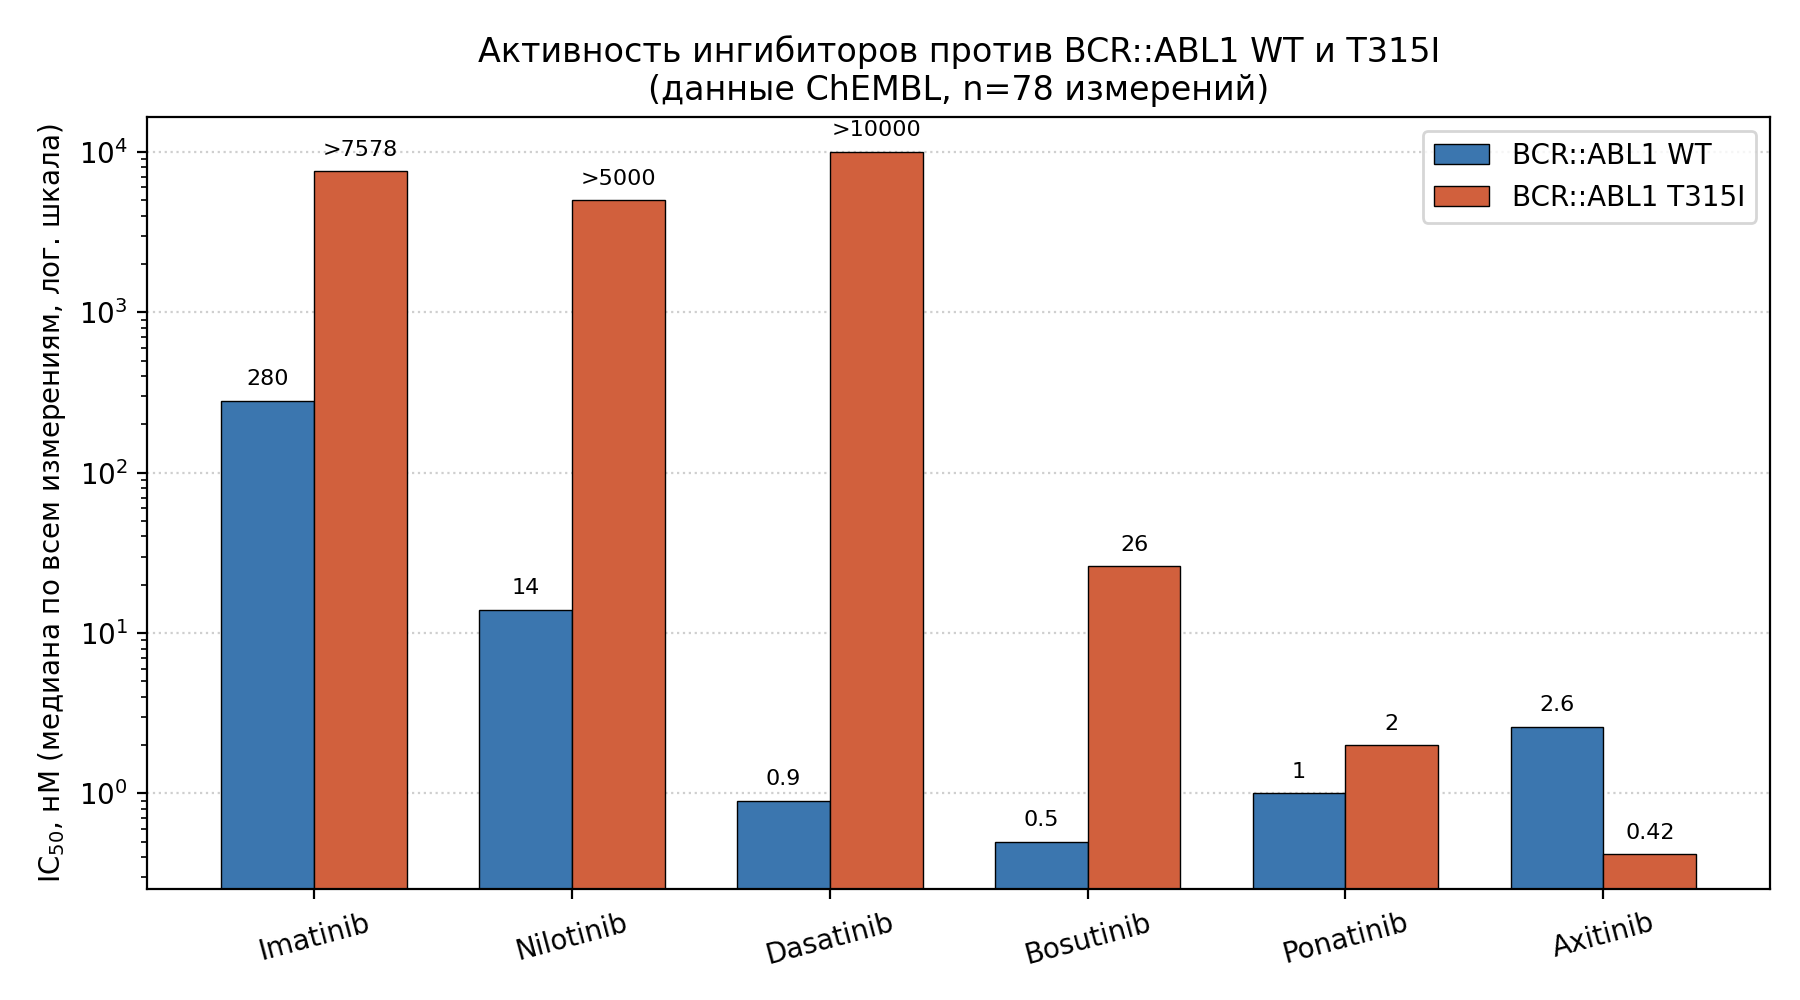
\includegraphics[width=\linewidth]{../figures/fig_activity.png}
\caption{Медианные значения IC$_{50}$ для каждого соединения по всем измерениям из
собранного набора данных; логарифмическая шкала. Знак «$>$» над столбцом означает, что
в число измерений входят цензурированные значения, то есть истинное IC$_{50}$ ещё выше.
Построено скриптом \code{scripts/plot\_activity.py} по файлу \code{BCR\_ABL\_dataset.csv}.}
\end{figure}

\medskip
\noindent\textbf{Краткая интерпретация графика.}
Для ингибиторов 1-го и 2-го поколений (иматиниб, нилотиниб, дазатиниб) переход от WT к
T315I увеличивает IC$_{50}$ на 1--4 порядка: наиболее драматично для дазатиниба,
у которого активность падает с ${\approx}0{,}9$ нМ до $>10\,000$ нМ. Бозутиниб занимает
промежуточное положение: потеря активности заметная (0{,}5 $\rightarrow$ 26 нМ), но
не катастрофическая, хотя клинически он против T315I всё равно не применяется.
У понатиниба разница между формами составляет менее одного порядка, а у аксетиниба
активность против мутанта даже \emph{выше}, чем против WT --- именно этот эффект стал
основанием рассматривать его как кандидата для перепрофилирования при T315I-резистентности.
График наглядно показывает, что T315I --- не «общее ухудшение связывания», а
избирательный эффект, зависящий от того, опирается ли конкретная молекула на контакт с
gatekeeper-остатком.

\section{Target Data Passport}

\begin{center}
\begin{tabular}{L{4.4cm}L{5.0cm}L{5.0cm}}
\toprule
\textbf{Параметр} & \textbf{BCR::ABL1 WT} & \textbf{BCR::ABL1 T315I} \\
\midrule
Исследуемый domain & ABL1 kinase domain, остатки 242--493 (UniProt P00519) & то же, ABL1 kinase domain 242--493 \\
Аминокислота 315 & Thr & Ile \\
PDB structures доступны? & да, 60 записей с киназным доменом & да, 8 записей (из них 4 --- человеческий ABL1) \\
Выбранный PDB ID & \textbf{2HYY} & \textbf{3QRJ} \\
Experimental method & X-ray diffraction & X-ray diffraction \\
Resolution & 2.40~\AA & 1.82~\AA \\
Ligand & STI --- иматиниб & 919 --- ребастиниб (DCC-2036) \\
Известные inhibitors & иматиниб, нилотиниб, дазатиниб, бозутиниб, понатиниб, асциминиб (все активны) & понатиниб, асциминиб; in~vitro также аксетиниб; TKI 1--2 поколений неактивны \\
Activity data доступны? & да: IC$_{50}$ и K$_d$, 42 измерения в собранном наборе & да, но частично цензурированы ($>5000$, $>10\,000$ нМ), 36 измерений \\
SMILES доступны? & да, для всех 7 соединений (PubChem) & да, те же соединения \\
Достаточно данных для дальнейшего modelling? & да & да, с оговорками (см. раздел~13) \\
\bottomrule
\end{tabular}
\end{center}

\section{Итоговый вывод}

\textbf{Достаточно ли доступных данных по BCR::ABL1 WT и T315I для дальнейшего
computational drug discovery?} В целом --- да, обе формы мишени обеспечены данными
достаточно, чтобы переходить к структурному анализу, докингу и хемоинформатике.

\medskip
\noindent\textbf{Структурные данные.} Достаточно. Для киназного домена ABL1 доступно
68 записей PDB, из них 60 соответствуют форме WT и 8 --- T315I; подавляющее большинство
получено рентгеновской дифракцией с разрешением 1{,}8--2{,}5~\AA. Выбранные структуры
2HYY (2{,}40~\AA) и 3QRJ (1{,}82~\AA) --- человеческий белок без посторонних мутаций,
с полностью разрешённым сайтом связывания.

\medskip
\noindent\textbf{Данные о лигандах.} Достаточно. Известно как минимум шесть одобренных
препаратов и десятки исследовательских соединений; 64 из 68 структур киназного домена
содержат связанную малую молекулу, то есть доступны экспериментальные позы лигандов ---
это позволит валидировать протокол докинга редокингом.

\medskip
\noindent\textbf{Activity data.} Достаточно, но требует осторожности. Собрано 78
измерений IC$_{50}$/K$_d$ из 11 первичных источников. Значения разнородны по
методике, и для T315I заметная часть данных цензурирована.

\medskip
\noindent\textbf{Chemical data.} Достаточно. Для всех соединений получены PubChem CID,
брутто-формула, молекулярная масса и SMILES (с учётом стереохимии), то есть данные
полностью машиночитаемы.

\medskip
\noindent\textbf{Обнаруженные ограничения и пробелы в данных:}
\begin{enumerate}[leftmargin=*,topsep=2pt,itemsep=3pt]
\item \textbf{Асимметрия по формам мишени.} Структур T315I в 7{,}5 раза меньше, чем WT
(8 против 60), а человеческих --- всего 4. Для мутанта выбор структуры практически
безальтернативен.
\item \textbf{Нет структуры полноразмерного BCR::ABL1.} Все экспериментальные данные
относятся к изолированному киназному домену ABL1; вклад BCR-части (олигомеризация,
дополнительные сайты фосфорилирования) структурно не охарактеризован.
\item \textbf{Цензурированные значения активности.} Для иматиниба, нилотиниба и
дазатиниба против T315I большинство величин --- это границы ($>5000$, $>10\,000$ нМ).
Для регрессионных моделей (QSAR) такие данные напрямую непригодны и требуют либо
отбрасывания, либо специальной обработки.
\item \textbf{Неоднородность анализов.} Разброс IC$_{50}$ одного соединения между
публикациями достигает двух порядков (иматиниб против WT: 75--7700 нМ). Смешивать такие
значения в одной обучающей выборке нельзя.
\item \textbf{Пробелы в ChEMBL.} Для асциминиба не нашлось записи активности с
явной пометкой T315I, хотя из литературы известно, что он сохраняет активность против
этого мутанта (аллостерический механизм). Это показывает, что автоматическая выгрузка
из базы не заменяет проверку по первичным публикациям.
\item \textbf{Нет AlphaFold-модели мутанта и слитного белка.} Модель T315I при
необходимости придётся строить самостоятельно.
\item \textbf{Разные системы нумерации остатков} (изоформы 1a/1b, мышиный ортолог) ---
источник ошибок при сопоставлении структур и литературных данных; при дальнейшей
работе нумерацию нужно проверять для каждой записи отдельно.
\end{enumerate}

\medskip
\noindent\textbf{Итог:} накопленных данных достаточно для следующих этапов курса.
Для дальнейшей работы фиксируются структуры \textbf{2HYY (WT)} и \textbf{3QRJ (T315I)}
и набор данных \code{BCR\_ABL\_dataset.csv} (78 измерений, 7 соединений).

\appendix
\section{Приложение. Скрипты для выгрузки данных}
\label{app:scripts}

Все выборки воспроизводимы; скрипты приложены в папке \code{scripts/}:

\begin{center}
\small
\begin{tabular}{L{5.0cm}L{9.5cm}}
\toprule
\textbf{Файл} & \textbf{Назначение} \\
\midrule
\code{fetch\_uniprot.py} & Выгрузка записи P00519 из UniProt REST; печать доменов, сайтов и остатка 315 \\
\code{survey\_pdb.py} & Поиск всех структур PDB со ссылкой на ABL1/Abl1, классификация WT/T315I по последовательности, подсчёт статистики \\
\code{fetch\_chembl.py} & Выгрузка активностей (IC$_{50}$, K$_i$, K$_d$) для 7 соединений против ChEMBL1862 и ChEMBL2096618 \\
\code{fetch\_pubchem.py} & Получение CID, формулы, MW и SMILES через PubChem PUG REST \\
\code{build\_dataset.py} & Сборка \code{BCR\_ABL\_dataset.csv} и \code{.xlsx} из выгруженных данных \\
\code{plot\_activity.py} & Построение графика \code{figures/fig\_activity.png} \\
\bottomrule
\end{tabular}
\end{center}

\section{Приложение. Состав сданных материалов}

\begin{center}
\small
\begin{tabular}{L{5.5cm}L{9.0cm}}
\toprule
\textbf{Файл} & \textbf{Описание} \\
\midrule
\code{report.pdf} / \code{report.tex} & Настоящий отчёт \\
\code{BCR\_ABL\_dataset.csv} & Набор данных, 78 строк (одна строка --- одно измерение) \\
\code{BCR\_ABL\_dataset.xlsx} & Тот же набор в формате Excel \\
\code{figures/fig\_activity.png} & Визуализация (раздел~11) \\
\code{scripts/} & Скрипты выгрузки и обработки данных \\
\code{data/} & Сырые выгрузки из ChEMBL, PubChem и RCSB (JSON) \\
\bottomrule
\end{tabular}
\end{center}

\vspace{1.5cm}
\noindent Выбранные PDB ID для дальнейших работ: \textbf{2HYY} (WT), \textbf{3QRJ} (T315I).

\vspace{1cm}
\noindent Подписи студентов: \underline{\hspace{5cm}} \hfill Дата: \underline{\hspace{3.5cm}}

\end{document}
